%\setcounter{chapter}{-1}
\chapter*{Introducción}

La teoría de Ecuaciones Diferenciales es la teoría matemática relacionada con el movimiento. Esta trata de resolver ecuaciones cuyas soluciones son funciones. Podríamos pensar en llamar a este área ``Ecuaciones Funcionales'', pero gracias a que en física $F = m \cdot a$, podemos encontrar de forma natural y útil ecuaciones funcionales donde la información que aparezca sobre la función a buscar está relacionada con las relaciones que guardan las derivadas de dicha función.

\begin{ejemplo}
    Como ejemplo de ecuación diferencial que surge de forma natural podemos pensar en el movimiento de un péndulo:

    Para describir un péndulo, nos es suficiente con tres variables independientes, que podemos ver en la siguiente ilustración:
    \begin{itemize}
        \item La longitud del hilo del péndulo, a la que llamamos $l$.
        \item La aceleración gravitatoria del planeta en el que nos encontremos, a la que llamamos $g$.
        \item Y el ángulo que guarda el péndulo sobre la vertical, al que llamamos $\theta$.
    \end{itemize}

    % Péndulo

\ifdefined\showimages
    \begin{figure}[H]
        \centering
        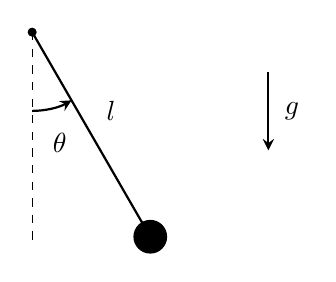
\begin{tikzpicture}
            % Parámetros
            \def\L{3}        % Longitud del péndulo
            \def\LL{2.7}     % Longitud de la vertical
            \def\ang{30}     % Ángulo del péndulo (en grados)
    
            % Dibujar la línea discontinua vertical
            \draw[dashed] (0,0) -- (0,-\LL);
    
            % Dibujar el péndulo
            \draw[thick] (0,0) -- ({\L*sin(\ang)}, {-\L*cos(\ang)});
    
            % Dibujar el círculo al final del péndulo
            \filldraw[thick] ({\L*sin(\ang)}, {-\L*cos(\ang)}) circle (0.2);
    
            % Indicar el ángulo
            \draw[thick, -stealth] (0,-1) arc[start angle=270, end angle=300, radius=1];
            \node at (0.35, -1.4) {$\theta$};
            \node at (1, -1) {$l$};
            \node at (3.3, -1) {$g$};

            % Flecha hacia abajo para la gravedad
            \draw[thick, -stealth] (3, -0.5) -- (3, -1.5);
    
            % Dibujar el punto de suspensión
            \filldraw (0,0) circle (0.05);
        \end{tikzpicture}
    \end{figure}
\fi
    Como nuestro objetivo es describir el movimiento que describe un péndulo, tenemos que introducir una variable más, el tiempo ($t$), y ver ahora la variable $\theta$ como una variable dependiente en función de $t$:
    \begin{equation*}
        \theta = \theta(t)
    \end{equation*}
    La física nos dice que si $\theta(t)$ es una función que nos describe el movimiento de un péndulo en función del tiempo, entonces debe cumplir la siguiente ecuación\footnote{De dónde sale dicha ecuación no nos es relevante.}:
    \begin{equation}\label{eq:pendulo}
        \theta''(t) + \frac{g}{l} \sen \theta(t) = 0
    \end{equation}

    A partir de esta ecuación, nos preguntamos por las funciones $\theta$ que cumplan dicha ecuación, siendo esta la primera ecuación diferencial que trataremos de resolver.

    A simple vista, podemos decir acertadamente que dos soluciones para dicha ecuación son:
    \begin{equation*}
        \theta(t) = 0 \qquad \qquad  \theta(t) = \pi
    \end{equation*}
    Pensando que en ambas soluciones el péndulo se encuentra en un estado estático, en la primera este se encuentra quieto debajo y en la segunda, quieto arriba. De forma intuitiva podemos pensar que el primero es un equilibrio estable y el segundo un equilibrio inestable.

    A partir de dichas soluciones, podemos adivinar que también serán soluciones de~(\ref{eq:pendulo}) cualquier función de la forma:
    \begin{equation*}
        \theta(t) = n\pi, \quad n \in \mathbb{Z}
    \end{equation*}
    De esta forma, hemos encontrado una \textbf{familia de soluciones}, es decir, tenemos una función que es solución de~(\ref{eq:pendulo}) para cada $n\in \mathbb{Z}$.

    Hemos encontrado infinitas soluciones para la ecuación~(\ref{eq:pendulo}). Podemos pensar que cada una de estas soluciones describe un péndulo distinto (esto es, cada una de las distintas formas de tirar el péndulo). En el mundo de las ecuaciones diferenciales es común encontrar muchas soluciones para una sola ecuación.

    En el caso de la ecuación~(\ref{eq:pendulo}), se ha demostrado que a parte de la familia de soluciones que hemos dado, no pueden encontrarse más soluciones con fórmula (aunque pueden aproximarse).
\end{ejemplo}~\\

El orden de una ecuación diferencial es la derivada de mayor grado que aparezca en la fórmula de la ecuación. En el caso de~(\ref{eq:pendulo}), esta era de orden 2. En esta asignatura nos centraremos en el estudio de las ecuaciones diferenciales de orden 1.

Una ecuación diferencial de primer orden genérica es de la forma:
\begin{equation}\label{eq_generica}
    \Phi(t,x(t), x'(t))=0
\end{equation}
Es decir, es una relación entre una variable independiente ($t$, que usualmente podremos entender como el tiempo), una variable dependiente o función ($x$, en función de $t$), cuya expresión estamos interesados en buscar; y su derivada.

La $\Phi$ que aparece en~(\ref{eq_generica}) será una función:
\Func{\Phi}{D\subseteq \mathbb{R}^3}{\mathbb{R}}{(t,x,y)}{\Phi(t,x,y)}
Donde trataremos de ver $x$ como variable independiente que tenemos que hacer dependiente de $t$: $x=x(t)$, siendo $y$ su derivada.

\begin{ejemplo}
    Dada la siguiente ecuación diferencial:
    \begin{equation*}
        {(x(t))}^{2} + {(x'(t))}^{2} = 1
    \end{equation*}
    La función $\Phi$ en cuestión es:
    \Func{\Phi}{D=\mathbb{R}^3}{\mathbb{R}}{(t,x,y)}{x^2+y^2-1}
    Soluciones de dicha ecuación son (a simple vista):

    \begin{equation*}
    \begin{array}{ll}
        x(t) = \sen t & x(t) = \cos t \\
        x(t) = 1 & x(t) = -1
    \end{array}
    \end{equation*}

    Además, podemos deducir que una familia de soluciones que engloba a las dos primeras es:
    \begin{equation*}
        x(t) = \sen(t+c), \quad c\in \mathbb{R}
    \end{equation*}

    % Grafica de familia de soluciones, 1 y -1
\ifdefined\showimages
    \begin{center}
    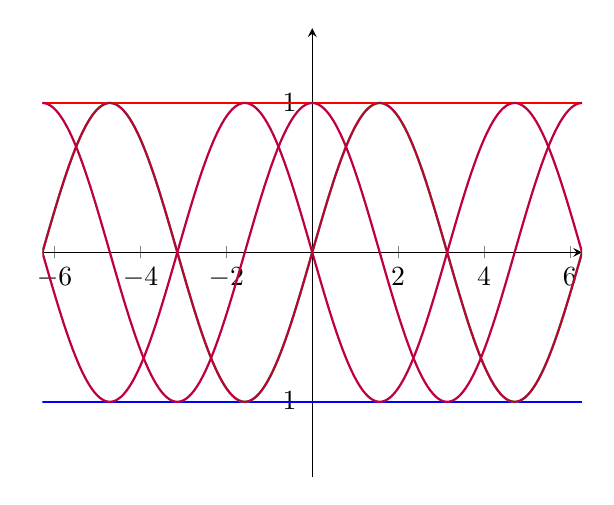
\begin{tikzpicture}
      \begin{axis}[
          axis lines = center,    % Dibujar los ejes
          xmin = -2*pi, xmax = 2*pi,   % Definir el rango en el eje x
          ymin = -1.5, ymax = 1.5,         % Definir el rango en el eje y
          xlabel = {},              % Etiqueta del eje x
          ylabel = {},                 % Etiqueta del eje y
          domain = -2*pi:2*pi,         % Dominio de las funciones
          samples = 200,               % Número de muestras para las funciones
          legend pos = north west,     % Posición de la leyenda
          %grid = both,                 % Mostrar la cuadrícula
          major grid style = {lightgray},   % Estilo de la cuadrícula principal
          minor grid style = {dotted}       % Estilo de la cuadrícula secundaria
      ]

      % Función constante 1
      \addplot[red, thick] {1};

      % Función constante -1
      \addplot[blue, thick] {-1};

      % Función sen(x)
      \addplot[green, thick] {sin(deg(x))};

      % Función cos(x)
      \addplot[purple, thick] {cos(deg(x))};

      % Función sen(x + pi)
      \addplot[purple, thick] {sin(deg(x + pi))};

      % Función sen(x + pi)
      \addplot[purple, thick] {sin(deg(x + 2 * pi))};

      \end{axis}
    \end{tikzpicture}
    \end{center}
\fi

    Graficando las soluciones, podemos además construir una nueva solución con una función a trozos:
    \begin{equation*}
        x(t) = \left\{\begin{array}{ll}
                \cos t & t \geq 0 \\
                1 & t<0
        \end{array}\right.
    \end{equation*}
    Derivable en $\mathbb{R}^*$ por el carácter local de la derivabilidad y en 0 por coincidir los dos límites laterales de las derivadas. Sin embargo, observamos que no es dos veces derivable.
\end{ejemplo}~\\

Las ecuaciones diferenciales de orden 1 sin restricción alguna son demasiado generales como para construir una teoría formal que centre su estudio en estas. Por tanto, estudiaremos aquellas que admitan escribirlas en \textbf{forma normal}, es decir, que si nos dan una ecuación en la forma~(\ref{eq_generica}), esta pueda escribirse como:
\begin{equation}\label{eq_generica_normal}
    x'(t) = f(t,x(t))
\end{equation}
Para una cierta
\Func{f}{C\subseteq \mathbb{R}^2}{\mathbb{R}}{(t,x)}{f(t,x)}

\begin{ejemplo}
    Dadas las dos siguientes ecuaciones diferenciales, discutir cuál de ellas es más simple y resolver ambas.
    \begin{itemize}
        \item $x'(t) = 7x(t)$
        \item $x'(t) = 7t$
    \end{itemize}
    La segunda ecuación es más sencilla, ya que se trata de un cálculo de una primitiva para $x'$: $x'(t) = h(t)$, a lo que ya estamos acostumbrados.

    Para dicha ecuación, tenemos:
    \begin{gather*}
        \Phi(t,x,y) = y-7t \\
        f(t,x) = 7t
    \end{gather*}

    con $D=\mathbb{R}^3$ y $C=\mathbb{R}^2$.

    Las soluciones de dicha ecuación diferencial son, por tanto:
    \begin{equation*}
        x(t) = \frac{7}{2} t^2 + c, \quad c\in \mathbb{R}
    \end{equation*}
    Para la primera ecuación, tenemos:
    \begin{gather*}
        \Phi(t,x,y) = y-7x \\
        f(t,x) = 7x
    \end{gather*}

    con $D=\mathbb{R}^3$ y $C=\mathbb{R}^2$.

    De forma simple vemos dos primeras soluciones:
    \begin{equation*}
        x(t) = 0 \qquad  x(t) = e^{7t}
    \end{equation*}

    Y podemos deducir además una familia de soluciones:
    \begin{equation*}
        x(t) = c \cdot e^{7t}, \quad c\in \mathbb{R}
    \end{equation*}

    De hecho, demostraremos más adelante que dicha ecuación no tiene más soluciones además de las de dicha familia.

\end{ejemplo}
   
\begin{ejemplo}
    Dadas las dos siguientes ecuaciones diferenciales, discutir cuál de ellas es más simple e intentar resolverlas.
    \begin{itemize}
        \item $x'(t) = \sen t$
        \item $x'(t) = \sen x(t)$
    \end{itemize}
    En este caso, es la primera la que es más simple, ya que se vuelve a tratar de un cálculo de primitiva.

    Tenemos:
    \begin{gather*}
        \Phi(t,x,y) = y-\sen t \\
        f(t,x) = \sen t
    \end{gather*}

    Siendo las soluciones de la ecuación diferencial:
    \begin{equation*}
        x(t) = -\cos t + c, \quad c \in \mathbb{R}
    \end{equation*}
    En el caso de la segunda, tenemos:
    \begin{gather*}
        \Phi(t,x,y) = y-\sen x \\
        f(t,x) = \sen x
    \end{gather*}
    Ecuación que todavía no sabemos resolver.
\end{ejemplo}
